% ARIN7600 final oral, about 40 minutes.
% Numbers follow the group final report
% (355020_Boyang_Pang_Final_Report_Group_122_...pdf).
% Histogram distances from different sections are not on one scale.
% Compile from this directory:
%   latexmk -pdf -interaction=nonstopmode -halt-on-error final_report.tex
\documentclass[aspectratio=169,11pt,t]{beamer}

\usefonttheme{professionalfonts}
\usepackage{lmodern}
\usepackage{booktabs}
\usepackage{amsmath,amssymb}
\usepackage{tikz}
\usetikzlibrary{arrows.meta,positioning}

\definecolor{HKUGreen}{RGB}{0,104,87}
\definecolor{HKUGreenDark}{RGB}{0,62,54}
\definecolor{HKULight}{RGB}{232,243,240}
\definecolor{HKUGrey}{RGB}{70,78,76}

\setbeamercolor{normal text}{fg=black,bg=white}
\setbeamercolor{structure}{fg=HKUGreen}
\setbeamercolor{frametitle}{fg=HKUGreenDark,bg=white}
\setbeamercolor{title}{fg=HKUGreenDark}
\setbeamercolor{itemize item}{fg=HKUGreen}
\setbeamercolor{itemize subitem}{fg=HKUGreenDark}
\setbeamercolor{enumerate item}{fg=HKUGreen}
\setbeamercolor{section in head/foot}{fg=white,bg=HKUGreenDark}
\setbeamercolor{section in head/foot shaded}{fg=HKULight!70,bg=HKUGreenDark}
\setbeamercolor{author in head/foot}{fg=white,bg=HKUGreenDark}
\setbeamercolor{title in head/foot}{fg=white,bg=HKUGreen}
\setbeamercolor{date in head/foot}{fg=white,bg=HKUGreenDark}
\setbeamercolor{block title}{fg=white,bg=HKUGreen}
\setbeamercolor{block body}{fg=black,bg=HKULight}
\setbeamercolor{block title alerted}{fg=white,bg=HKUGreenDark}
\setbeamercolor{block body alerted}{fg=black,bg=HKULight}

\setbeamerfont{frametitle}{series=\bfseries,size=\large}
\setbeamerfont{section in head/foot}{size=\scriptsize,series=\bfseries}
\setbeamerfont{author in head/foot}{size=\scriptsize}
\setbeamerfont{title in head/foot}{size=\scriptsize}
\setbeamerfont{date in head/foot}{size=\scriptsize}
\setbeamersize{text margin left=7mm,text margin right=7mm}
\setbeamertemplate{navigation symbols}{}
\hypersetup{hidelinks}

\graphicspath{{../kpp_ks/kpp_report/figs/}}
% A tabular is an inline box. Without these breaks, the next sentence
% continues on the table's baseline and collides with the rows.
\BeforeBeginEnvironment{tabular}{\par}
\AfterEndEnvironment{tabular}{\par}

\setbeamertemplate{headline}{%
  \begin{beamercolorbox}[wd=\paperwidth,ht=2.7ex,dp=1.05ex]{section in head/foot}%
    \insertsectionnavigationhorizontal{\paperwidth}{\hskip0.55em}{\hskip0.55em}%
  \end{beamercolorbox}%
}

\setbeamertemplate{frametitle}{%
  \vspace{0.15em}%
  \insertframetitle\par
  \vspace{0.12em}%
  {\color{HKUGreen}\rule{\textwidth}{0.7pt}}\par
  \vspace{0.15em}%
}

\setbeamertemplate{footline}{%
  \leavevmode%
  \hbox{%
    \begin{beamercolorbox}[wd=.34\paperwidth,ht=2.6ex,dp=1.1ex,leftskip=1em]{author in head/foot}%
      \usebeamerfont{author in head/foot}Group 12.2%
    \end{beamercolorbox}%
    \begin{beamercolorbox}[wd=.46\paperwidth,ht=2.6ex,dp=1.1ex,center]{title in head/foot}%
      \usebeamerfont{title in head/foot}ARIN7600 \quad Two-Step Diffusion%
    \end{beamercolorbox}%
    \begin{beamercolorbox}[wd=.20\paperwidth,ht=2.6ex,dp=1.1ex,rightskip=1em]{date in head/foot}%
      \usebeamerfont{date in head/foot}\hfill\insertframenumber\,/\,\inserttotalframenumber%
    \end{beamercolorbox}%
  }%
}

\newcommand{\sectime}{}
\AtBeginSection[]{%
  \begin{frame}[plain]
    \vfill
    {\color{HKUGreen}\rule{2.4cm}{2.2pt}}\par\vspace{0.7em}
    {\color{HKUGreen}\Large\bfseries \insertsectionnumber}\par\vspace{0.2em}
    {\Huge\bfseries \insertsection}\par\vspace{0.55em}
    {\color{HKUGrey}\large \sectime}\par
    \vfill
  \end{frame}%
}

\newcommand{\pipeline}{%
  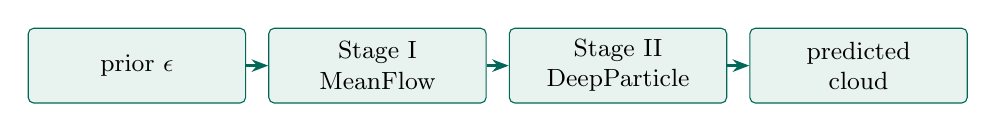
\begin{tikzpicture}[
      node distance=0.28cm,
      box/.style={draw=HKUGreen,fill=HKULight,rounded corners=2pt,
                  minimum height=0.95cm,text width=2.55cm,align=center,
                  font=\small,inner sep=3pt},
      arr/.style={-{Stealth[length=2.1mm]},HKUGreen,very thick}
    ]
    \node[box] (prior) {prior $\epsilon$};
    \node[box,right=of prior] (s1) {Stage I\\ MeanFlow};
    \node[box,right=of s1] (s2) {Stage II\\ DeepParticle};
    \node[box,right=of s2] (out) {predicted\\ cloud};
    \draw[arr] (prior) -- (s1);
    \draw[arr] (s1) -- (s2);
    \draw[arr] (s2) -- (out);
  \end{tikzpicture}%
}

\title{Two-Step Diffusion}
\subtitle{Particle surrogates for Keller--Segel, KPP, and Fokker--Planck}
\author{YANG Zhenyu \and PANG Boyang \and LIU Jialin}
\institute{The University of Hong Kong\\ MSc in Artificial Intelligence}
\date{27 November 2026}

\begin{document}

% ----- title -----
\begin{frame}[plain]
  \begin{tikzpicture}[remember picture,overlay]
    \fill[HKUGreen] (current page.north west) rectangle ([yshift=-1.9cm]current page.north east);
    \fill[HKUGreenDark] (current page.south west) rectangle ([yshift=1.45cm]current page.south east);
    \node[anchor=north west,text=white,font=\small] at ([xshift=0.85cm,yshift=-0.42cm]current page.north west)
      {The University of Hong Kong};
    \node[anchor=north west,text=HKULight,font=\scriptsize] at ([xshift=0.85cm,yshift=-1.05cm]current page.north west)
      {Master of Science in Artificial Intelligence \quad ARIN7600};
    \node[anchor=south,text=white,font=\scriptsize,align=center] at ([yshift=0.32cm]current page.south)
      {Group 12.2 \quad YANG Zhenyu \quad PANG Boyang \quad LIU Jialin\\[0.18em]
       Supervisor: Prof.\ Zhiwen Zhang, Department of Mathematics \quad 27 November 2026};
  \end{tikzpicture}
  \vspace{2.15cm}
  \begin{center}
    {\LARGE\bfseries Two-Step Diffusion}\\[0.45em]
    {\large A forty-minute report on particle generation}\\[0.35em]
    {\color{HKUGrey} Keller--Segel, KPP, and Fokker--Planck}\\[1.15em]
    \pipeline
  \end{center}
  \note{Open by naming the course and the claim: two network evaluations replace the particle solver at test time.}
\end{frame}

\begin{frame}{Forty minutes}
  \begin{tabular}{@{}clp{7.6cm}@{}}
    \toprule
    & Part & What it has to establish \\
    \midrule
    5 min & Introduction & The task, the pipeline, and the four headlines \\
    7 min & DeepParticle & Wasserstein matching, and why it is local \\
    8 min & Two-step diffusion & One global step, then a frozen corrector \\
    13 min & Three equations & Keller--Segel, KPP, Fokker--Planck \\
    4 min & Two parameters & Continuity in $(\sigma,\mu)$ \\
    3 min & Future work & The gap, and the next experiments \\
    \bottomrule
  \end{tabular}

  \vspace{0.7em}
  \begin{alertblock}{The sentence to leave with}
    Stage~I moves the cloud onto the right support.
    Stage~II, trained by mini-batch optimal transport, pulls the mass into place.
    At inference the particle solver is not called.
  \end{alertblock}
  \note{Read the clock once. Say that the three equations share this pipeline, and that their distances are not one number.}
\end{frame}

% ============================================================
\renewcommand{\sectime}{About five minutes}
\section[Introduction]{Introduction}

\begin{frame}{High-fidelity clouds are expensive}
  Interacting particles are a flexible solver for nonlinear diffusion, aggregation, and front speeds.
  The object we actually need is often the \emph{terminal cloud}, or a long-time invariant measure, at many values of a physical parameter.
  \vspace{0.6em}
  \begin{itemize}
    \item A Keller--Segel trajectory integrates interaction, advection, and noise out to a fixed horizon.
    \item A KPP front speed waits through thousands of Feynman--Kac generations.
    \item The same family of clouds is required again at the next parameter value.
  \end{itemize}
  \vspace{0.5em}
  The solver stays in the training pipeline.
  The question is whether a network can emit the cloud when the solver is no longer affordable.
  \note{Do not apologise for the solver. It is the teacher of the network.}
\end{frame}

\begin{frame}{What the surrogate is asked to do}
  \centering
  \pipeline

  \vspace{0.7em}
  \begin{columns}[T,onlytextwidth]
    \begin{column}{0.48\textwidth}
      \textbf{Training}\\[0.3em]
      \raggedright
      An interacting-particle method builds a reference cloud for each condition $\eta$.
      Stage~I learns a one-step transport from a simple prior.
      Stage~II freezes that map and learns a small correction.
    \end{column}
    \begin{column}{0.48\textwidth}
      \textbf{Inference}\\[0.3em]
      \raggedright
      Draw $\epsilon$ from the prior, evaluate Stage~I once, evaluate Stage~II once.
      The output is a particle cloud at the requested $\eta$.
      No time step, no resampling, no chemotaxis sum.
    \end{column}
  \end{columns}
  \note{Point at the four boxes left to right. Emphasise that the solver is absent from the right-hand column.}
\end{frame}

\begin{frame}{What this project contributes}
  The source paper studies three-dimensional Keller--Segel and KPP, and does not release a complete implementation.
  This capstone rebuilds the architecture and then moves it.
  \vspace{0.45em}
  \begin{itemize}
    \item Laminar and Kolmogorov Keller--Segel, with the advection amplitude as the condition.
    \item KPP front speeds on the two-torus and on the three-torus.
    \item A new target: a Fokker--Planck double well, with and without spatial killing.
    \item A continuity argument for conditioning on shear and diffusivity together.
  \end{itemize}
  \vspace{0.35em}
  A class-conditional sampler for handwritten digits is a separate check that the target need not come from a PDE.
  It returns at the end.
  \note{Four contributions. Save the digit experiment so it does not compete with the equations.}
\end{frame}

\begin{frame}{Each distance has its own ruler}
  Every number below is a quadratic Wasserstein distance on a histogram.
  The binning, the projection, and the number of seeds change with the equation.
  \vspace{0.4em}
  \small
  \begin{tabular}{@{}llp{5.7cm}@{}}
    \toprule
    Experiment & Ruler & How to hear it \\
    \midrule
    Laminar KS & 16 bins per axis, 3 seeds & The benchmark table \\
    Kolmogorov KS & Histogram, one seed & Interim; not the 16-bin table \\
    KPP on $\mathbb{T}^2$ & $72\times 72$, periodic & About $0.13$, not $0.19$ \\
    KPP on $\mathbb{T}^3$ & $W_2$ of the $x$--$z$ projection & A shadow of the cloud \\
    Fokker--Planck & $96\times 96$ & Compared with a self-distance \\
    \bottomrule
  \end{tabular}
  \vspace{0.45em}
  \normalsize
  A smaller number is better \emph{inside one row}.
  A $0.13$ on the torus is not a better laminar result than $0.19$.
  \note{This slide prevents the usual question that adds the tables together. Stay on it until that is clear.}
\end{frame}

\begin{frame}{The headlines, before the details}
  \small
  \begin{tabular}{@{}lccc@{}}
    \toprule
     & Initialiser & Two-step & What changes \\
    \midrule
    Laminar KS, 20 amplitudes & $0.3545$ & $0.1902$ & $46.35\%$ lower \\
    Kolmogorov KS, full test & $0.19152$ & $0.14270$ & $25.49\%$ lower \\
    KPP on $\mathbb{T}^2$, 11 levels & $0.1434$ & $0.1345$ & lower on 8 of 11 \\
    KPP on $\mathbb{T}^3$, $x$--$z$ & $0.1293$ & $0.1065$ & lower on 10 of 11 \\
    \bottomrule
  \end{tabular}
  \vspace{0.55em}
  \normalsize
  On the laminar row the initialiser is MeanFlow, and DeepParticle alone sits at $0.4564$, worse than MeanFlow.
  On the Kolmogorov row the initialiser is improved MeanFlow.
  Fokker--Planck has no single mean in the report: the two-step cloud is closer at every plotted strength of the potential.
  \note{Read only the laminar percentage slowly. Say the other rows are the same pattern on a different ruler.}
\end{frame}

% ============================================================
\renewcommand{\sectime}{About seven minutes}
\section[DeepParticle]{DeepParticle}

\begin{frame}{The object is a cloud, not a labelled list}
  A reference at condition $\eta$ is an empirical measure
  \[
    \hat\rho_N=\frac1N\sum_{i=1}^N\delta_{X_i}.
  \]
  The network returns another cloud of $N$ points.
  Nothing in the sampler tells us which generated point is supposed to match which reference point.
  \vspace{0.45em}
  \begin{itemize}
    \item The prior and the target are drawn independently.
    \item A particle index is an arbitrary label.
    \item A pointwise mean square would change if either cloud were reordered.
  \end{itemize}
  \note{One concrete picture: two identical clouds, written in different order, must have distance zero.}
\end{frame}

\begin{frame}{Quadratic Wasserstein distance}
  For measures $\mu$ and $\nu$,
  \[
    W_2^2(\mu,\nu)
    =\inf_{\gamma\in\Gamma(\mu,\nu)}\int\|x-y\|_2^2\,\mathrm{d}\gamma(x,y).
  \]
  On two equal-weight clouds the same definition is a linear program over couplings,
  \[
    \widehat W_2^2
    =\min_{\gamma\in\Gamma_N}\sum_{i,j}\gamma_{ij}\,\|x_i-y_j\|_2^2,
    \qquad
    \gamma\ge 0,\;
    \gamma\mathbf{1}=\tfrac1N\mathbf{1},\;
    \gamma^\top\mathbf{1}=\tfrac1N\mathbf{1}.
  \]
  \vspace{0.35em}
  The cost sees mass and geometry.
  It does not see the order of the lists.
  Exact solution of this program is the Earth Mover's distance.
  \note{Say coupling in one sentence: a joint plan whose row and column sums recover the two clouds.}
\end{frame}

\begin{frame}{How DeepParticle uses that distance}
  DeepParticle learns a deterministic map by minimising the empirical Wasserstein distance to particle data.
  The original method alternates two updates:
  \vspace{0.4em}
  \begin{enumerate}
    \item Move the network parameters, with the current coupling held fixed.
    \item Recompute the coupling, with the network held fixed.
  \end{enumerate}
  \vspace{0.45em}
  The first papers in this line target an invariant measure, then a finite-time Keller--Segel cloud, then a map that can also be run backwards.
  In the two-step algorithm the same idea is used more narrowly.
  Stage~I is expected to have done the global displacement, so the transport plan only has to finish a local alignment.
  \note{Name Wang, Xin, and Zhang, 2022 and 2024, without reading the titles.}
\end{frame}

\begin{frame}{Where the reference cloud comes from}
  Before either network is trained, a particle method turns the PDE into points.
  \vspace{0.35em}
  \begin{itemize}
    \item Keller--Segel: Euler--Maruyama on an interacting system with a smoothed attraction kernel, a prescribed flow, and Brownian noise.
    \item KPP: a genetic algorithm on the torus. Each generation advances one forcing period, reweights by a Feynman--Kac potential, and resamples.
    \item Fokker--Planck: for the double well, equilibrium points can be drawn from the Gibbs law directly, because the potential factors.
  \end{itemize}
  \vspace{0.4em}
  The stored cloud is the teacher.
  Training does not rerun the long particle system at every step.
  \note{The three constructions return in part four. Here the audience only needs to know that the teacher is a point cloud.}
\end{frame}

\begin{frame}{A corrector that starts as the identity}
  After Stage~I is frozen, the second map is
  \[
    f_\phi(x,\eta)=x+\alpha\, h_\phi(x,\eta).
  \]
  The last layer of $h_\phi$ is initialised at zero, so the first prediction is exactly $x$.
  \vspace{0.4em}
  For a mini-batch of Stage~I points and a condition-matched reference batch, the cost matrix is
  \[
    C_{ij}=\|f_\phi(x_i,\eta)-x^{\mathrm{ref}}_j\|_2^2.
  \]
  An exact Earth Mover's solve on that batch produces a coupling $\gamma$.
  The loss is the transport cost plus a penalty that keeps the step small,
  \[
    \mathcal{L}_{\mathrm{DP}}
    =\langle C,\gamma\rangle
    +\frac{\lambda_{\mathrm{res}}}{B}\sum_{i=1}^B\|f_\phi(x_i,\eta)-x_i\|_2^2.
  \]
  \note{The residual term is why we call the second map a corrector. Without it, nothing stops a second global rearrangement.}
\end{frame}

\begin{frame}{The coupling is exact, and it is stale on purpose}
  The full cloud is too large for an Earth Mover's solve at every step.
  The method therefore does three different things on three clocks.
  \vspace{0.35em}
  \begin{itemize}
    \item The default Stage~II run has $20{,}000$ parameter updates.
    \item The mini-batch is redrawn every $1{,}500$ updates.
    \item The coupling is recomputed every $50$ updates, by an exact solve on the current batch.
  \end{itemize}
  \vspace{0.4em}
  Between solves, $\gamma$ is a constant.
  The loss can fall smoothly and then jump when the plan is replaced.
  That jump is the schedule.
  Mini-batch optimal transport is also a biased stand-in for the distance on the full cloud, which is accepted so that the exact solve remains possible.
  \note{If asked why not Sinkhorn: the training target in this project is the exact mini-batch coupling.}
\end{frame}

\begin{frame}{Alone, the corrector is a weak global map}
  On the laminar Keller--Segel sweep the same 16-bin distance, averaged over $\sigma=10,20,\ldots,200$ and over seeds $88$, $89$, and $90$, is
  \vspace{0.35em}
  \begin{center}
  \begin{tabular}{lccc}
    \toprule
    MeanFlow & DeepParticle alone & MeanFlow $+$ DP & Reduction from MeanFlow \\
    \midrule
    $0.3545$ & $0.4564$ & $0.1902$ & $46.35\%$ \\
    \bottomrule
  \end{tabular}
  \end{center}
  \vspace{0.35em}
  DeepParticle alone is lower than MeanFlow only at $\sigma\in\{10,70,80,90\}$.
  It does not build the sheared support.
  Once MeanFlow has placed that support, the corrector is lower than both one-stage maps at every amplitude.
  \note{This is the reason for two stages. Do not read it as a failure of optimal transport. Read it as the wrong job for a near-identity map.}
\end{frame}

% ============================================================
\renewcommand{\sectime}{About eight minutes}
\section[Two-Step]{Two-Step Diffusion}

\begin{frame}{One global move, then a local repair}
  Flow matching learns an instantaneous velocity.
  Integrating that velocity still costs many network evaluations.
  MeanFlow replaces the velocity by its average over a time interval, and the whole transport collapses to one evaluation.
  \vspace{0.45em}
  That one evaluation is fast, and it is a weak instrument for fine geometry.
  DeepParticle has the opposite profile: an explicit Wasserstein loss, and no mechanism that first carries mass across the domain.
  \vspace{0.45em}
  \begin{block}{The split}
    Stage~I is a one-step MeanFlow map from the prior onto the support.
    Stage~II is a DeepParticle corrector, trained only after Stage~I is frozen.
  \end{block}
  \note{Say coarse, then fine. The freeze is a design choice, and it returns as a limitation.}
\end{frame}

\begin{frame}{Average velocity over an interval}
  Let $v$ be an instantaneous velocity and write $z_t$ for the state at time $t$.
  The average velocity from $r$ to $t$ is
  \[
    u(z_t,r,t)=\frac{1}{t-r}\int_r^t v(z_\tau,\tau)\,\mathrm{d}\tau,
    \qquad 0\le r<t\le 1.
  \]
  Differentiating in the upper limit gives the MeanFlow identity
  \[
    u(z_t,r,t)
    =v(z_t,t)-(t-r)\,\frac{\mathrm{d}}{\mathrm{d}t}u(z_t,r,t).
  \]
  The total derivative is a Jacobian--vector product,
  \[
    \frac{\mathrm{d}}{\mathrm{d}t}u
    =\mathrm{JVP}\big[u;\,(z_t,r,t);\,(v,0,1)\big].
  \]
  \note{If the room is mathematical, stay on the identity. If not, say: the network is trained to predict the displacement of a whole interval, not the slope at one instant.}
\end{frame}

\begin{frame}{The path, the target, and the one evaluation}
  Time runs from the target toward the prior.
  A target point $x_0$ and a prior point $\epsilon$ give
  \[
    z_t=(1-t)\,x_0+t\,\epsilon,
    \qquad
    v_c=\epsilon-x_0.
  \]
  The regression target replaces $v$ by $v_c$ and stops the gradient through the derivative,
  \[
    u_{\mathrm{tar}}=v_c-(t-r)\,\mathrm{JVP}.
  \]
  When $r=t$ the identity reduces to ordinary flow matching.
  A fixed fraction of the batch is placed on that boundary.
  \vspace{0.35em}
  The trained sampler does not integrate. From noise at time $1$,
  \[
    x_{\mathrm{MF}}=\epsilon-u_\theta(\epsilon,0,1,\eta).
  \]
  The physical condition $\eta$ enters as a sinusoidal embedding.
  It does not change the identity.
  It does ask one network to carry a family of transports.
  \note{Write the sampler formula on the board if you can. It is the whole of Stage I at test time.}
\end{frame}

\begin{frame}{Stage I, as it is trained}
  \small
  \begin{enumerate}
    \item Draw a condition $\eta$, a reference point $x_0$, a prior point $\epsilon$, and times $0\le r\le t\le 1$.
    \item Form the straight path $z_t$ and the conditional velocity $v_c=\epsilon-x_0$.
    \item For original MeanFlow, evaluate $u_\theta$ and its total derivative by a forward Jacobian--vector product. Set $u_{\mathrm{tar}}=v_c-(t-r)\dot u$ and regress $u_\theta$ toward the stopped target.
    \item Improved MeanFlow rearranges the same identity so that the regression target is the instantaneous velocity, which does not depend on the network. The Kolmogorov experiment uses this variant. The laminar table uses the original loss.
    \item Pixel MeanFlow is specified as a later ablation. It is not in the reported runs.
  \end{enumerate}
  \note{Do not derive improved MeanFlow. The only fact the later slides need is which experiment used which loss.}
\end{frame}

\begin{frame}{Stage II, after the first map is frozen}
  \begin{enumerate}
    \item Freeze $\theta$. Generate a Stage~I cloud for every training condition and keep the matched reference.
    \item Zero the last layer, so $f_\phi$ begins as the identity.
    \item On each step, map the current mini-batch through $f_\phi$.
    \item Every $50$ steps, rebuild the cost and replace $\gamma$ by the exact mini-batch coupling.
    \item Every $1{,}500$ steps, draw a new mini-batch.
    \item Update $\phi$ by the sum of the transport cost and the residual penalty.
  \end{enumerate}
  \vspace{0.35em}
  The Kolmogorov run reported later shortens this second stage to $10{,}000$ updates and sets its learning rate to $10^{-4}$.
  The $20{,}000$ / $50$ / $1{,}500$ rhythm is the default method, not a claim that every table used it.
  \note{Separate the algorithm from the run. Questions about the Kolmogorov learning rate should land here.}
\end{frame}

\begin{frame}{Inference is two evaluations}
  \[
    \epsilon
    \;\longmapsto\;
    x_{\mathrm{MF}}=\epsilon-u_\theta(\epsilon,0,1,\eta)
    \;\longmapsto\;
    \hat x=f_\phi(x_{\mathrm{MF}},\eta).
  \]
  \vspace{0.2em}
  \begin{columns}[T,onlytextwidth]
    \begin{column}{0.48\textwidth}
      \textbf{Present at training}\\[0.25em]
      \raggedright
      the particle solver,
      the reference clouds,
      the Jacobian--vector product,
      and the Earth Mover's solve.
    \end{column}
    \begin{column}{0.48\textwidth}
      \textbf{Present at inference}\\[0.25em]
      \raggedright
      one forward pass of $u_\theta$,
      one forward pass of $f_\phi$,
      and the requested condition $\eta$.
    \end{column}
  \end{columns}
  \vspace{0.45em}
  Both maps are deterministic.
  Changing $\eta$ changes the cloud without a new solve.
  \note{Close the method part on this formula. The next section tests it, for about thirteen minutes.}
\end{frame}

% ============================================================
\renewcommand{\sectime}{About thirteen minutes}
\section[Equations]{Three Equations}

\begin{frame}{One pipeline, three laws}
  \begin{columns}[T,onlytextwidth]
    \begin{column}{0.31\textwidth}
      \begin{block}{Keller--Segel}
        Aggregation in a prescribed flow.
        Laminar shear, then a cellular Kolmogorov field.
        The condition is the amplitude $\sigma$.
      \end{block}
    \end{column}
    \hfill
    \begin{column}{0.31\textwidth}
      \begin{block}{KPP}
        A reaction--diffusion front in a periodic flow.
        The learned object is the invariant measure that carries the front speed.
      \end{block}
    \end{column}
    \hfill
    \begin{column}{0.31\textwidth}
      \begin{block}{Fokker--Planck}
        A double well in the plane.
        First the equilibrium.
        Then the same well with a killing field.
      \end{block}
    \end{column}
  \end{columns}
  \vspace{0.55em}
  Kolmogorov flow is a second velocity in the Keller--Segel equation, not a fourth equation.
  \note{Gesture three columns. Spend the thirteen minutes as about four, five, and four.}
\end{frame}

\begin{frame}{Keller--Segel in three dimensions}
  The density of cells satisfies
  \[
    \partial_t\rho+v\cdot\nabla\rho
    =\mu\Delta\rho+\chi\nabla\cdot\big(\rho\,\nabla(K*\rho)\big).
  \]
  The regularised particle system used to build the teacher is
  \[
    \mathrm{d}X_i
    =-\frac{\chi}{N}\sum_{j\neq i}\nabla K_\delta(X_i-X_j)\,\mathrm{d}t
    +v(X_i)\,\mathrm{d}t
    +\sqrt{2\mu}\,\mathrm{d}W_i,
  \]
  with $K_\delta(z)=|z|/\big(4\pi(|z|^2+\delta^2)\big)$.
  \vspace{0.25em}
  In the laminar benchmark only the amplitude varies,
  \[
    v(x,y,z)=\sigma\big(e^{-y^2-z^2},\,0,\,0\big)^\top,
    \qquad \mu=1,
  \]
  and $\sigma=10,20,\ldots,200$.
  \note{Read the velocity as a shear along $x$ that is strongest near the $y=z=0$ axis. $\mu$ and $\chi$ stay fixed in this section.}
\end{frame}

\begin{frame}{Laminar sweep: the corrector wins at every amplitude}
  Exact 16-bin histogram $W_2$, mean of seeds $88$, $89$, and $90$.
  \vspace{0.3em}
  \small
  \begin{tabular}{@{}lcccc@{}}
    \toprule
    $\sigma$ & MeanFlow & DeepParticle & MeanFlow$+$DP & Reduction \\
    \midrule
    $10$  & $0.3411$ & $0.1809$ & $0.1509$ & $55.76\%$ \\
    $80$  & $0.2253$ & $0.2137$ & $0.1411$ & $37.37\%$ \\
    $140$ & $0.3384$ & $0.5182$ & $0.1699$ & $49.79\%$ \\
    $200$ & $0.8517$ & $1.1372$ & $0.4090$ & $51.98\%$ \\
    \midrule
    Mean of all $20$ & $0.3545$ & $0.4564$ & $0.1902$ & $46.35\%$ \\
    \bottomrule
  \end{tabular}
  \vspace{0.4em}
  \normalsize
  MeanFlow$+$DP is below both one-stage maps at all twenty amplitudes.
  Past $\sigma=140$ every error grows. The two-step curve stays the lowest.
  In the $x$--$z$ plane the reference becomes a sheared triangle; MeanFlow finds that support, DeepParticle alone stays rounded, and the corrector keeps the shear.
  \note{Do not read all twenty rows. The four rows show a weak shear, a moderate shear, and the two hard amplitudes. Offer the full table if asked.}
\end{frame}

\begin{frame}{The same equation in Kolmogorov flow}
  The velocity is replaced by
  \[
    v(x,y,z)=\sigma\big(\sin 2\pi z,\,\sin 2\pi x,\,\sin 2\pi y\big)^\top.
  \]
  Training uses $\sigma=10,20,\ldots,100$, and $\sigma=110$ is held out.
  The run is improved MeanFlow for $50{,}000$ steps, then $10{,}000$ corrector steps at learning rate $10^{-4}$.
  \vspace{0.35em}
  \small
  \begin{tabular}{@{}lccc@{}}
    \toprule
    Subset & iMF & iMF$+$DP & Reduction \\
    \midrule
    Training grid & $0.18183$ & $0.13314$ & $26.78\%$ \\
    Interpolation   & $0.18401$ & $0.13720$ & $25.44\%$ \\
    Extrapolation, $\sigma=110$ & $0.26659$ & $0.19772$ & $25.83\%$ \\
    Full test & $0.19152$ & $0.14270$ & $25.49\%$ \\
    \bottomrule
  \end{tabular}
  \vspace{0.35em}
  \normalsize
  The corrector removes about a quarter of the error on the grid, inside it, and at $\sigma=110$.
  One seed, and this generator predates the split between the Gaussian prior and the physical initial cloud.
  \note{Give the extrapolation row the stress. Then say the caveat in one breath, so the number is not quoted later as a three-seed result.}
\end{frame}

\begin{frame}{KPP: the front speed is stored as a cloud}
  On a periodic flow the reaction--diffusion equation is
  \[
    \partial_t u+v\cdot\nabla u=\kappa\Delta u+r u(1-u).
  \]
  The minimal speed in a direction $e$ is a variational eigenvalue,
  \[
    c^*(e)=\inf_{\lambda>0}\frac{\mu(\lambda)}{\lambda}.
  \]
  At fixed $\lambda$ the eigenvalue is carried by a twisted diffusion.
  On the two-torus that diffusion is
  \[
    \mathrm{d}X_t
    =\big(2\kappa\lambda e_1+v(X_t,t)\big)\,\mathrm{d}t+\sqrt{2\kappa}\,\mathrm{d}W_t.
  \]
  \vspace{0.25em}
  We store the long-time empirical measure, not the front itself.
  Here $\sigma=\kappa$, $\lambda=2$, and $\theta=1$.
  Training runs through $-\log_2\sigma=3.75$. Evaluation continues to $4.50$, so the last three levels are extrapolations.
  \note{Translate once: a good initial cloud for the particle system is a warm start for the speed. The cloud is the object the network learns.}
\end{frame}

\begin{frame}{The two-dimensional ridge}
  \centering
  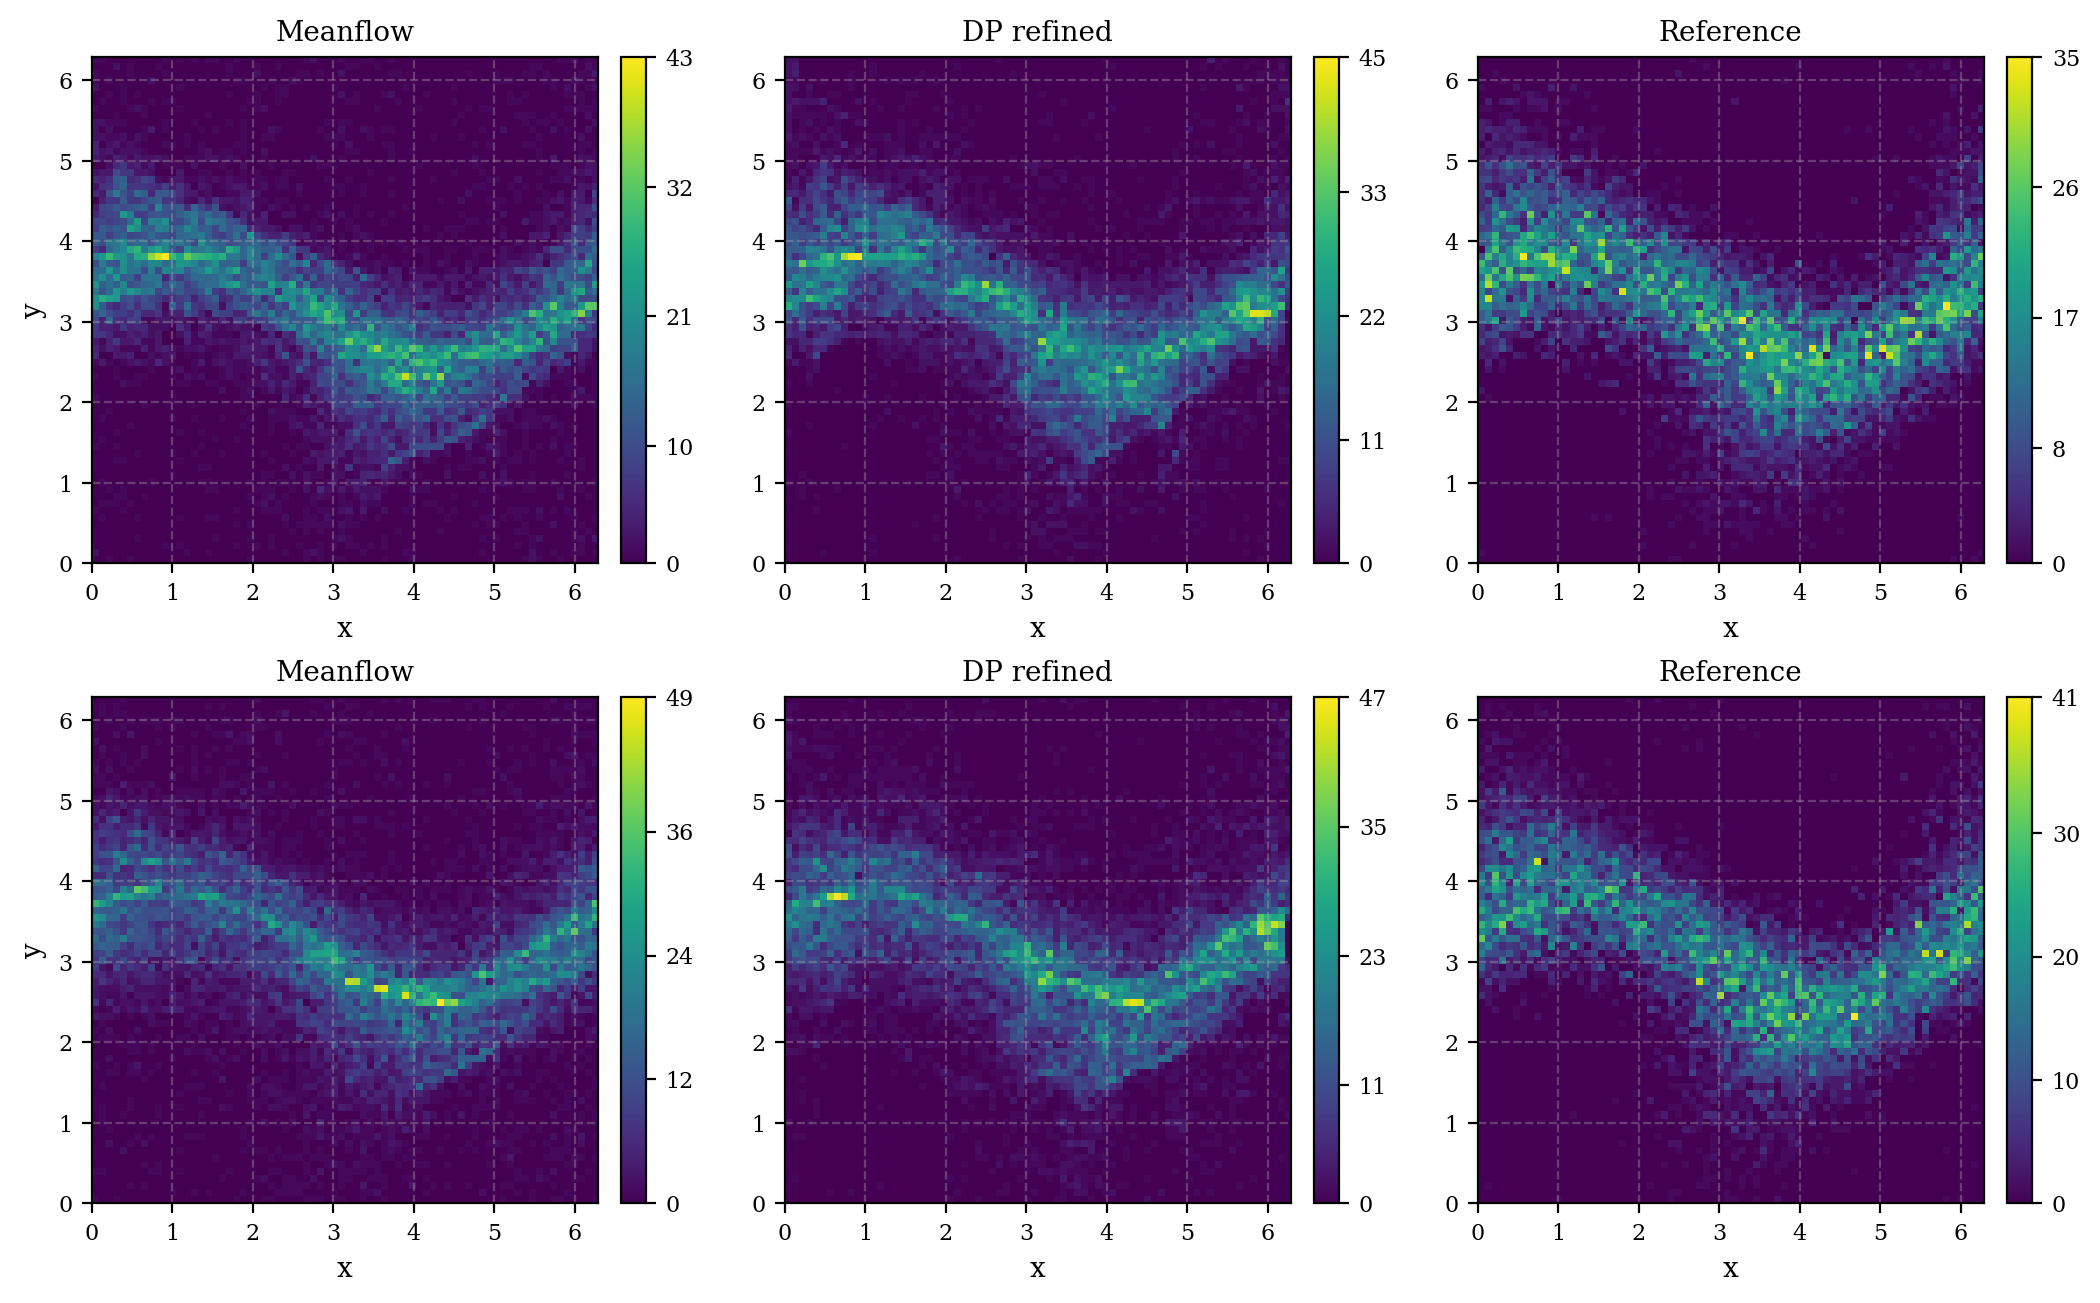
\includegraphics[height=0.62\textheight]{fig5_invariant_2d.png}\\[0.2em]
  {\scriptsize Top row: training level $\sigma=2^{-3.75}$.
  Bottom row: extrapolation $\sigma=2^{-4}$.
  Columns: MeanFlow, corrector, Feynman--Kac reference.
  Each panel has its own colour scale.}
  \note{Point at the wavy band. MeanFlow finds the trough. The reference is grainier. The corrector does not leave the band. The miss, where there is one, is geometric.}
\end{frame}

\begin{frame}{Two-dimensional distance and speed}
  A uniform cold start stays between $W_2=1.0538$ and $1.1718$ on the eleven-level grid.
  \vspace{0.3em}
  \begin{center}
  \begin{tabular}{lcc}
    \toprule
    $-\log_2\sigma$ & MeanFlow & Corrector \\
    \midrule
    $2.00$ (coarsest training) & $0.0962$ & $0.1061$ \\
    $3.75$ (end of training) & $0.1424$ & $0.1368$ \\
    $4.50$ (farthest extrapolation) & $0.2629$ & $0.2326$ \\
    \midrule
    Mean of all $11$ & $0.1434$ & $0.1345$ \\
    \bottomrule
  \end{tabular}
  \end{center}
  \vspace{0.3em}
  The corrector is lower on eight of the eleven levels, including all three extrapolations.
  The source paper's MeanFlow mean is $0.0769$, and its value at $-\log_2\sigma=4.50$ is $0.0456$.
  The shape of our curve matches the training boundary: the error is quiet inside the range and rises beyond it.
  The absolute gap to the source paper is still open.
  \note{Say $1.05$ down to $0.14$ first, against the cold start. Then say the corrector is a smaller step, and the paper is still lower.}
\end{frame}

\begin{frame}{Three-dimensional invariant measure at $\sigma=2^{-4.5}$}
  \centering
  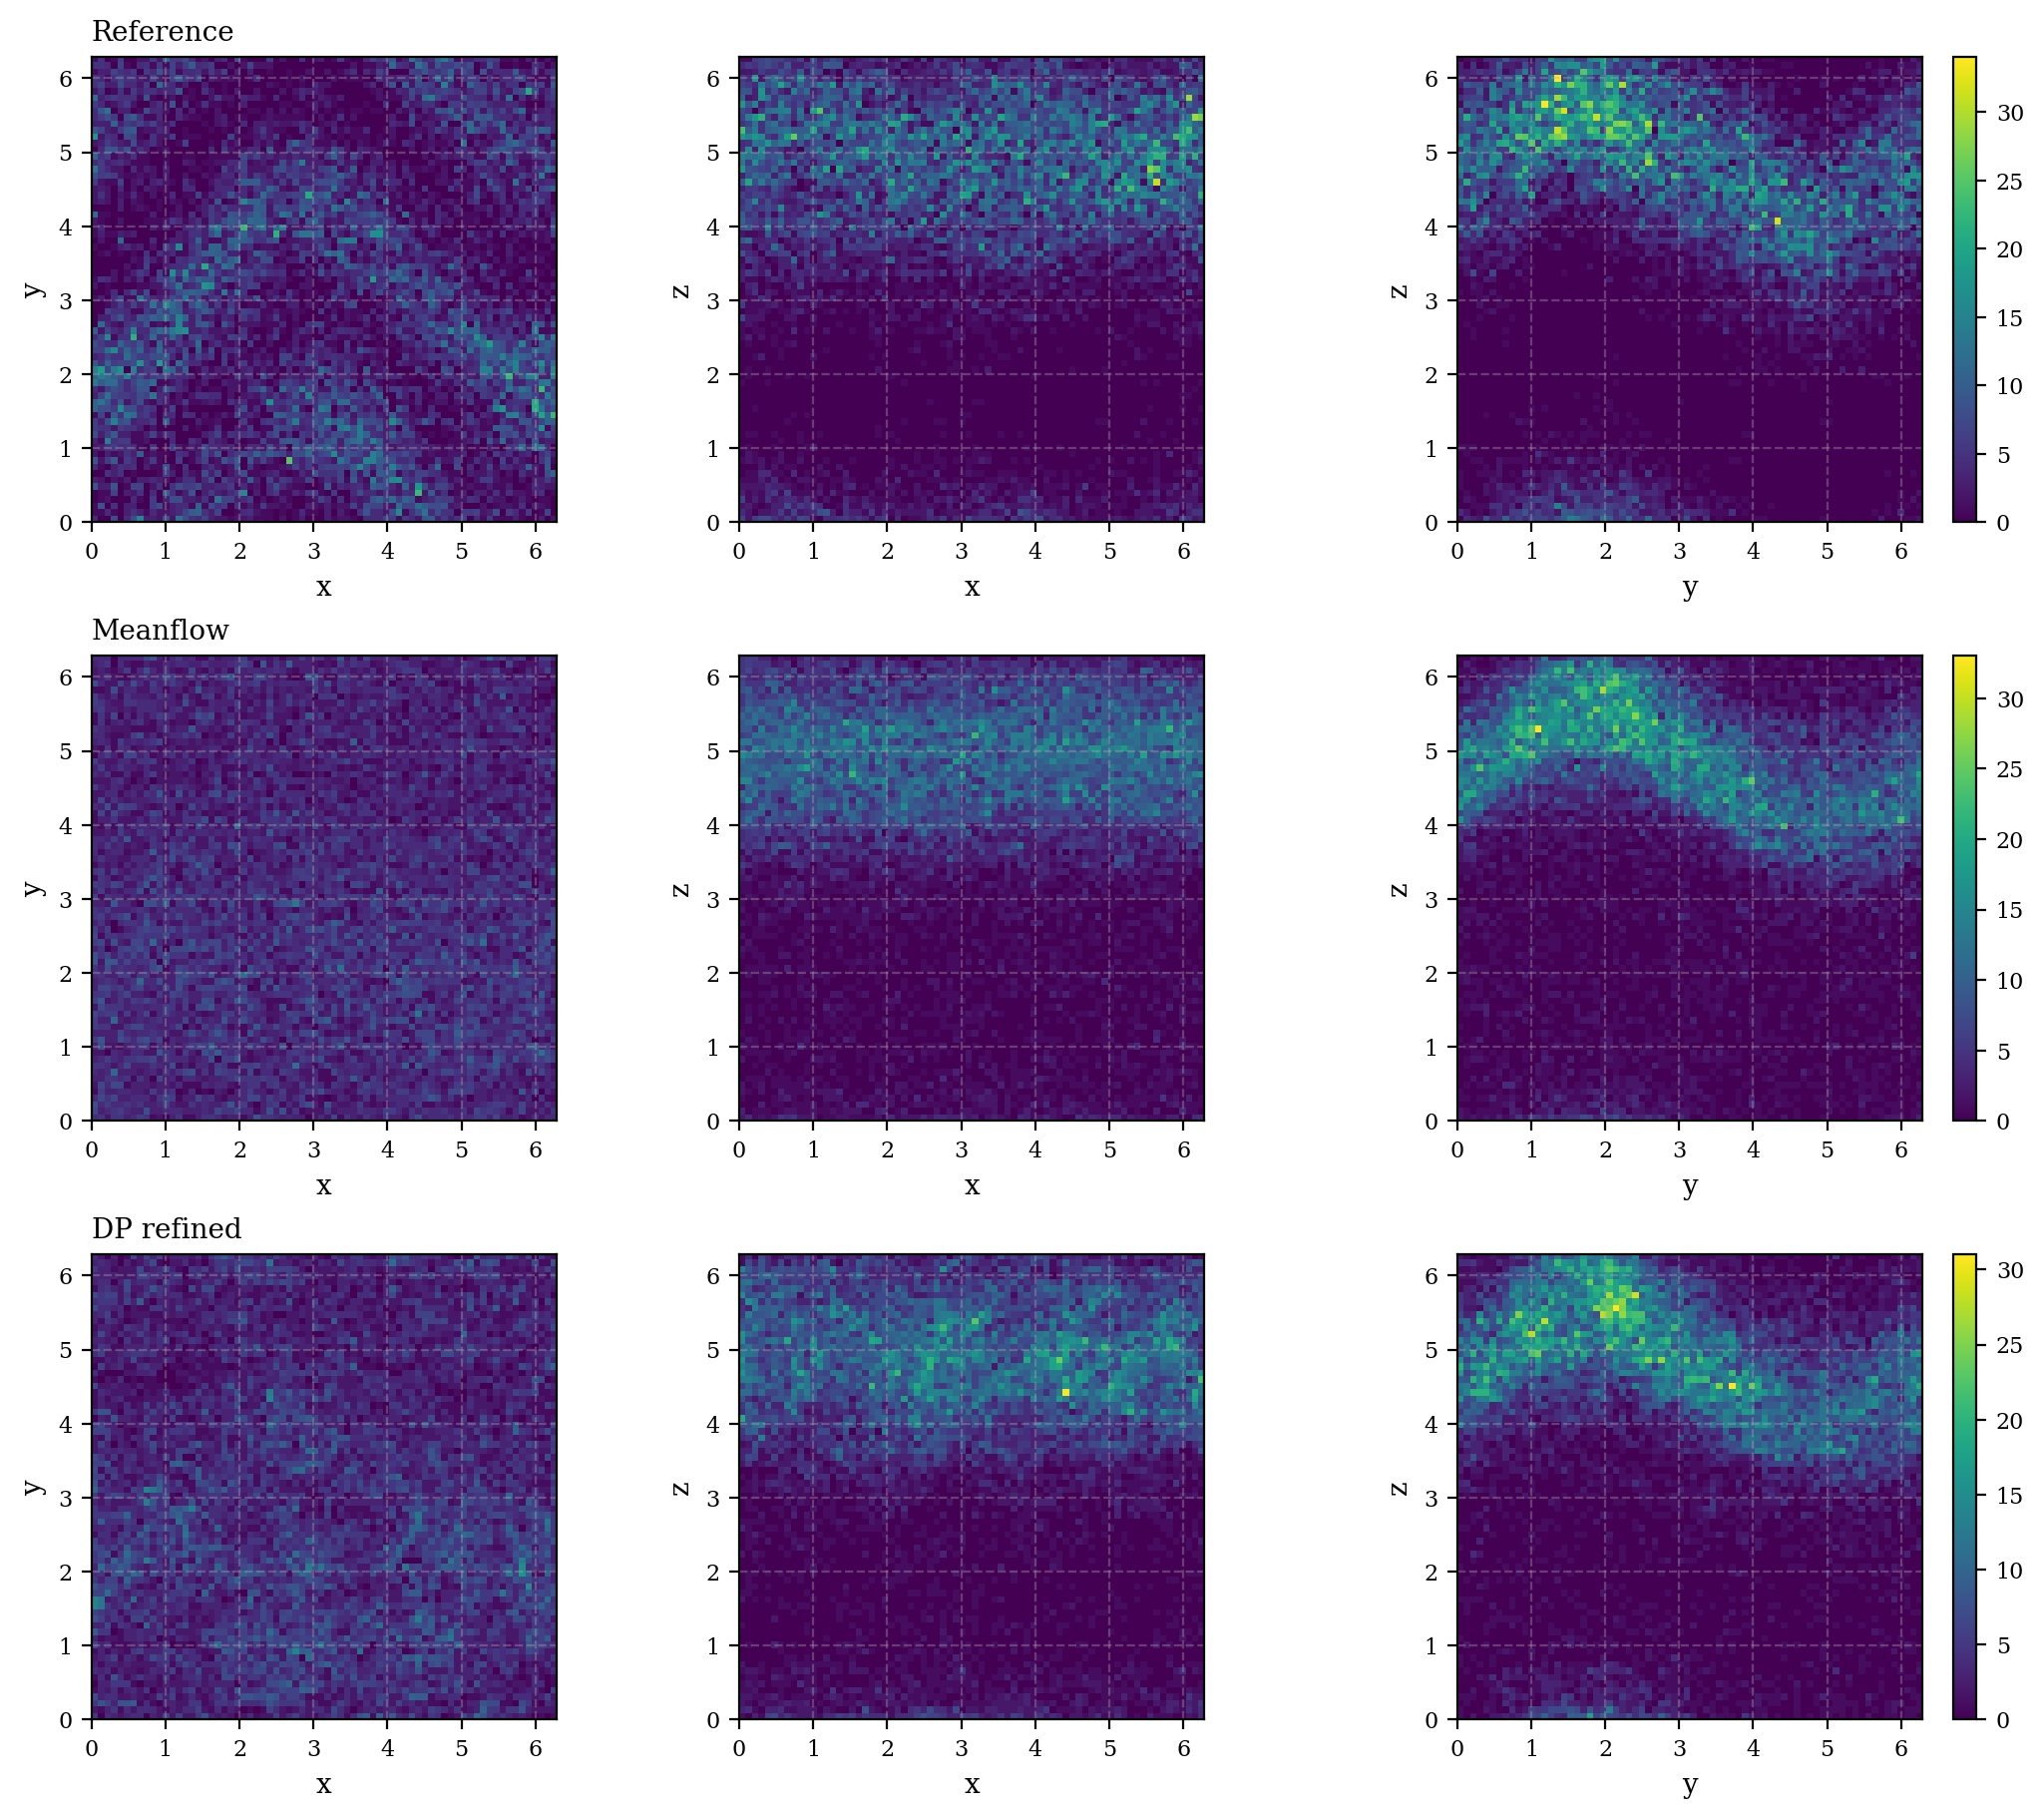
\includegraphics[height=0.62\textheight]{fig8_projections_3d.png}\\[0.15em]
  {\scriptsize Columns: $x$--$y$, $x$--$z$, $y$--$z$.
  The distance on the next slide uses the middle column.}
  \note{The middle column is the scored one. MeanFlow already has the high-$z$ mass. The corrector makes the $y$--$z$ ridge thinner and restores the two chevrons in $x$--$y$. Both generated clouds stay grainier than the reference.}
\end{frame}

\begin{frame}{Three-dimensional distance and speed}
  The velocity is the time-dependent Kolmogorov field
  \[
    v(x,t)=\big(
      \sin(x_3+\sin 2\pi t),\;
      \sin(x_1+\sin 2\pi t),\;
      \sin(x_2+\sin 2\pi t)
    \big),
  \]
  which is divergence-free at every $t$.
  The cold-start projection stays between $0.8895$ and $0.9600$.
  \vspace{0.3em}
  \begin{center}
  \small
  \begin{tabular}{lcc}
    \toprule
     & MeanFlow & Corrector \\
    \midrule
    Mean projected $W_2$ & $0.1293$ & $0.1065$ \\
    Source paper, same mean & $0.1312$ & $0.0294$ \\
    At $-\log_2\sigma=4.50$ & $0.1582$ & $0.1366$ \\
    \bottomrule
  \end{tabular}
  \end{center}
  \vspace{0.25em}
  \normalsize
  Our MeanFlow column sits next to the paper.
  Our corrector improves ten of the eleven levels, and it does not reach the paper's corrector.
  The smallest corrector error on the grid is $0.0920$, at $-\log_2\sigma=2.75$.
  \note{This is the cleanest comparison in the KPP section. MeanFlow is reproduced. The second stage is only partly reproduced.}
\end{frame}

\begin{frame}{A matching speed is not a resolved ridge}
  At $\sigma=2^{-4.5}$ the long-horizon Feynman--Kac speeds are $\hat c=0.7842$ in two dimensions and $0.6147$ in three.
  \vspace{0.35em}
  \small
  \begin{tabular}{@{}lcccc@{}}
    \toprule
     & Cold start & MeanFlow, $T=1$ & MeanFlow, $T=128$ & Corrector, $T=128$ \\
    \midrule
    $\mathbb{T}^2$ & near $0.51$ & $0.8180$ & $0.7841$ & $0.7848$ \\
    $\mathbb{T}^3$ & near $0.36$ & $0.6148$ & $0.6131$ & $0.6142$ \\
    \bottomrule
  \end{tabular}
  \vspace{0.45em}
  \normalsize
  A uniform cloud needs on the order of $10^2$ generations to reach the reference speed.
  The learned warm start is already there, and in three dimensions it is there at the first generation.
  The histogram error at the same states is still of order $10^{-1}$.
  The log-weight estimator forgives a ridge that is too smooth.
  The Wasserstein distance does not.
  \note{This is the slide to slow down on. A warm start can be right for the speed and still be the wrong shape.}
\end{frame}

\begin{frame}{Fokker--Planck in a double well}
  Rotate the plane by $\pi/4$ and write $(s,u)^\top=R_{\pi/4}^\top x$.
  With diffusion $D=0.2$ and well strength $a>0$,
  \[
    V_a(x)=a\left[\frac{(s^2-1)^2}{4}+\left(u-\frac{s}{2}\right)^2\right],
    \qquad
    \mathrm{d}X_t=-\nabla V_a(X_t)\,\mathrm{d}t+\sqrt{2D}\,\mathrm{d}B_t.
  \]
  The minima sit at $(s,u)=\pm(1,1/2)$.
  The barrier at the origin is $a/4$ above either minimum, so a larger $a$ makes two sharper peaks and a harder crossing.
  \vspace{0.3em}
  Without killing, the stationary law is the Gibbs density proportional to $e^{-V_a/D}$.
  Those points are sampled directly.
  Eight geometric strengths from $a=0.25$ to $a=4$ are used for training, seven midpoints for interpolation, and $a\in\{0.2,4.5,5\}$ for extrapolation.
  \note{The new content relative to the source paper starts on this slide. Say so.}
\end{frame}

\begin{frame}{Equilibrium, killing, and the spectral gap}
  On a $96\times 96$ histogram the two-step cloud has lower mean $W_2$ than MeanFlow at every plotted training strength and every plotted test strength.
  A paired self-distance of independent reference clouds is the soft floor: an exact sampler would not score zero under this binning.
  \vspace{0.4em}
  The spectral gap is a second test.
  Both models track it through the maximum near $a=0.45$ and the later decline.
  At $a=5$ they still estimate a gap above $0.03$, against a finite-volume benchmark near $0.0035$.
  The shape can look right while the relaxation rate is too fast.
  \vspace{0.4em}
  With the killing field $\kappa_a(x)=A(a)\,[1+\tanh(s/2)]$, calibrated so the two basins hold mass in a ratio near $0.3$, both generators reproduce the asymmetry.
  The two-step refinement again lowers the histogram distance across the tested strengths.
  \note{Do not invent a mean $W_2$ for this section. The report gives the ordering and the gap, not one summary distance.}
\end{frame}

% ============================================================
\renewcommand{\sectime}{About four minutes}
\section[Two Parameters]{Two Parameters}

\begin{frame}{Interpolation needs a continuous target}
  In the Keller--Segel experiments above, the network sees only $\sigma$.
  Diffusivity $\mu$ and the chemotactic strength stay fixed.
  Replacing the condition by $\eta=(\sigma,\mu)$ is legitimate only if the terminal cloud itself moves continuously.
  \vspace{0.4em}
  Let $\theta=(\sigma,\mu)$ and let $\nu_\theta$ be the laminar terminal cloud.
  Training on a finite set of cells, and evaluating a cell in between, requires
  \[
    \theta\;\longmapsto\;\nu_\theta
  \]
  to be continuous in the same 16-bin histogram $W_2$ used to score the learned map.
  A jump would put neighbouring parameters a finite distance apart, and no interpolation of the sampled cells would be meaningful.
  \note{This section is about the teacher, before any network. Say that in the first sentence if the title is misread as another accuracy table.}
\end{frame}

\begin{frame}{The modulus suggested by the particle system}
  Couple two copies of the Keller--Segel particles to the same initial cloud and the same Brownian motion.
  The shear enters linearly in $\sigma$.
  The diffusion coefficient is $\sqrt{2\mu}$, so that direction is square-root H\"older and is the weaker of the two.
  The resulting modulus is
  \[
    W_2(\nu_{\theta_1},\nu_{\theta_2})
    \le L\Big(|\sigma_1-\sigma_2|+\sqrt{|\mu_1-\mu_2|}\Big).
  \]
  \vspace{0.4em}
  This is the claim the next table is built to test.
  It is not a curve fitted to the measurements.
  The interaction kernel is fixed, and at the regularisation used here it does not change the form of the modulus.
  \note{Lipschitz in $\sigma$, square-root in $\mu$. The table will not estimate $L$. It will show that the distance falls as the step falls.}
\end{frame}

\begin{frame}{A local test around $(\sigma,\mu)=(100,1)$}
  Same $10^5$ initial particles. The distance is the 16-bin histogram $W_2$.
  Two clouds at one $\theta$ sit at a floor of $0.0644$.
  The step is $h=|\Delta\log_{10}\theta|$, and the last column removes that floor in quadrature.
  \vspace{0.45em}
  \small
  \begin{tabular}{@{}llccc@{}}
    \toprule
    Direction & Neighbour & $h$ & $W_2$ & Corrected$/h$ \\
    \midrule
    $\sigma$, at $\mu=1$ & $\sigma=110$ & $0.0414$ & $0.1874$ & $4.25$ \\
    $\sigma$, at $\mu=1$ & $\sigma=105$ & $0.0212$ & $0.1309$ & $5.38$ \\
    $\sigma$, at $\mu=1$ & $\sigma=102.5$ & $0.0107$ & $0.0922$ & $6.16$ \\
    $\mu$, at $\sigma=100$ & $\mu=2$ & $0.3010$ & $0.1466$ & $0.437$ \\
    $\mu$, at $\sigma=100$ & $\mu=1.5$ & $0.1761$ & $0.1019$ & $0.449$ \\
    $\mu$, at $\sigma=100$ & $\mu=1.25$ & $0.0969$ & $0.0723$ & $0.338$ \\
    \bottomrule
  \end{tabular}
  \vspace{0.45em}
  \normalsize
  $W_2$ falls as $h$ falls. The ratio stays within a factor $1.45$ along $\sigma$ and $1.33$ along $\mu$.
  A jump would send that ratio to infinity.
  \note{The last $\mu$ step is only $0.008$ above the floor. A finer $\mu$ step would not be visible in this histogram. Say that before someone asks for one.}
\end{frame}

\begin{frame}{What continuity licenses}
  Stage~I and Stage~II are compositions of continuous layers in $(\log_{10}\sigma,\log_{10}\mu)$.
  Every cloud they can represent moves continuously with the condition.
  \vspace{0.4em}
  \begin{itemize}
    \item If $\nu_\theta$ jumped, that function class would be the wrong class. Matching the sampled cells would not control the cells between them.
    \item The measurement says the laminar teacher does not jump, on the same 16-bin distance the network is scored by.
    \item The $\sigma$ direction is the steep one. The measured ratios along $\sigma$ are about an order of magnitude larger than those along $\mu$.
  \end{itemize}
  \vspace{0.35em}
  Continuity makes interpolation a meaningful request.
  It does not by itself choose how densely to sample a direction that is ten times steeper than the other.
  \note{Hand off to future work on the last sentence. Do not quote a joint-model accuracy from a different note.}
\end{frame}

% ============================================================
\renewcommand{\sectime}{About three minutes}
\section[Outlook]{Future Work}

\begin{frame}{Where the reproduction is still short}
  The two-step map improves on its own Stage~I in every experiment above.
  It does not yet sit on the lowest numbers reported for the source method.
  \vspace{0.4em}
  \begin{itemize}
    \item Laminar error grows for $\sigma\ge 140$, and the absolute level remains above the source paper.
    \item On KPP, the three-dimensional MeanFlow column is close to the paper. The corrector is not, and the extrapolated two-dimensional ridge is still several times too far.
    \item Generated KPP ridges are smoother than the Feynman--Kac grain.
    \item At a high double-well barrier the spectral gap is still estimated near $0.03$ instead of near $0.0035$.
  \end{itemize}
  \note{Own the gap. The positive sentence is the first one, and it is only a comparison with our own Stage I.}
\end{frame}

\begin{frame}{What we would change next}
  \begin{itemize}
    \item Retune Stage~I, and select checkpoints on a held-out distance, before asking the corrector to hide a weak initialiser.
    \item Sample $(\sigma,\mu)$, and later $(\sigma,\mu,\chi)$, by the curvature of the response. A uniform grid spends too many cells on the flat $\mu$ direction.
    \item Run the Pixel MeanFlow ablation that the method section already specifies.
    \item Try a prior other than a standard Gaussian, and a joint fine-tune in which Stage~I is not frozen for good.
    \item Keep an exact coupling, and test a randomised block solver against the mini-batch Earth Mover's step.
    \item Rerun the interim Kolmogorov and ablation studies after the prior is separated from the physical initial cloud.
  \end{itemize}
  \note{If time is short, say the first two items only: a better Stage I, and a design that respects the steep direction.}
\end{frame}

\begin{frame}{A target that is not a PDE}
  The same particle transport can be aimed at a shape.
  We fix a set of $28\times 28$ handwritten digits, keep pixels brighter than $0.15$, jitter them, and place them in $[-1,1]^2$.
  \vspace{0.4em}
  \begin{itemize}
    \item One network is shared across classes. The physical parameter is replaced by a learned embedding of dimension $24$.
    \item Inference takes $16$ equal steps. This check does not use the one-evaluation sampler of the PDE experiments.
    \item The cloud is drawn back to an image by a Gaussian kernel density on the pixel centres.
  \end{itemize}
  \vspace{0.4em}
  The sampler reproduces the digit it was shown.
  That is a lower bar than a font, and it is enough to show that the teacher of the cloud need not be a velocity field.
  A natural next question is a cloud that has to \emph{act}, rather than a cloud that has to look like a picture.
  \note{Ten seconds of pictures if you have them. Otherwise one sentence: the particles draw the digit, they do not classify it.}
\end{frame}

\begin{frame}{What we can defend today}
  \begin{enumerate}
    \item A frozen one-step MeanFlow map, followed by a near-identity optimal-transport corrector, emits a parameter-conditioned cloud with two evaluations.
    \item On laminar Keller--Segel that composition lowers the 16-bin distance from $0.3545$ to $0.1902$, and it is the best of the three maps at every amplitude.
    \item On KPP the same warm start reaches the front speed in a few generations, while the shape error shows that the ridge is not yet the reference ridge.
    \item The laminar teacher depends continuously on $(\sigma,\mu)$, with the steeper response in $\sigma$. Interpolation is a well-posed request. A uniform grid is not yet a good design.
  \end{enumerate}
  \vspace{0.55em}
  \begin{center}
    {\color{HKUGreen}\large\bfseries Questions}
  \end{center}
  \note{Stop. Do not add a fifth result in the answers unless it is already on a slide.}
\end{frame}

\begin{frame}{References}
  \small
  \begin{enumerate}
    \item Z.~Shen, Z.~Wang, J.~Xin, Z.~Zhang.
          Two-step diffusion: fast sampling and reliable prediction for 3D Keller--Segel and KPP equations in fluid flows.
          arXiv:2601.20024, 2026.
    \item Z.~Geng, M.~Deng, X.~Bai, J.~Z.~Kolter, K.~He.
          Mean flows for one-step generative modeling.
          arXiv:2505.13447, 2025.
    \item Z.~Geng, Y.~Lu, Z.~Wu, E.~Shechtman, J.~Z.~Kolter, K.~He.
          Improved mean flows.
          arXiv:2512.02012, 2026.
    \item Z.~Wang, J.~Xin, Z.~Zhang.
          DeepParticle: learning invariant measure by a deep neural network minimizing Wasserstein distance.
          \emph{J.\ Comput.\ Phys.}~464, 111309, 2022.
    \item Z.~Wang, J.~Xin, Z.~Zhang.
          A DeepParticle method for aggregation patterns in Keller--Segel systems.
          \emph{Physica D}~460, 134082, 2024.
    \item H.~Risken.
          \emph{The Fokker--Planck Equation.}
          Springer, 1996.
  \end{enumerate}
  \note{Leave this slide down unless a citation is requested.}
\end{frame}

\end{document}
